\documentclass[11pt,a4paper]{article}
\usepackage[T1]{fontenc}
\usepackage[utf8]{inputenc}
\usepackage{lmodern}
\usepackage[margin=2.3cm]{geometry}
\usepackage{graphicx}
\usepackage{booktabs}
\usepackage{longtable}
\usepackage{array}
\usepackage{xcolor}
\usepackage{hyperref}
\usepackage{caption}
\usepackage{float}
\usepackage{enumitem}

\hypersetup{colorlinks=true,linkcolor=blue!50!black,urlcolor=blue!50!black}
\setlist{itemsep=1pt,topsep=2pt}
\captionsetup{font=small,labelfont=bf}
\newcommand{\code}[1]{\texttt{\small #1}}
\newcolumntype{L}[1]{>{\raggedright\arraybackslash}p{#1}}

\title{\textbf{Wildfire Monitoring}\\[2pt]
\large Multi-source ingestion and analysis system for anomalous fire activity in Colombia\\[10pt]
\normalsize Workshop No.~1 --- Hazard Definition, Source Validation, and Data Contract}
\author{César Ospina (20222020059) \and Santiago Alfonso (20222020093) \and Adrián Espinosa (20222020104)\\
\normalsize Team 3 --- Computer Engineering, Universidad Distrital Francisco José de Caldas\\
\normalsize Data Analysis Programming --- Semester 2026-II}
\date{}

\begin{document}
\maketitle

\begin{abstract}
\noindent
This report formalises the first stage of a multi-source system that monitors vegetation fires in
Colombia and decides whether current fire activity is unusual relative to historical patterns
\emph{and} weather conditions. Four sources were selected, queried for real and profiled:
the NASA FIRMS active-fire archive, the Open-Meteo ERA5 historical weather API, the NASA FIRMS
near-real-time VIIRS stream (NOAA-20 and NOAA-21), and the Open-Meteo forecast API. The four
sources were validated on \textbf{703\,633} archived detections and \textbf{49\,170} region-days of
weather data. The profiling produced nine concrete data-quality problems, five verified
cross-sensor record pairs describing the same real event, and one quantified instrument
discontinuity: VIIRS detects \textbf{8.8$\times$} more records than MODIS for the same period, so a
baseline that mixes sensors manufactures an anomaly that does not exist. Only \textbf{33.7\,\%}
of the records returned by the Colombian bounding box are actually Colombian. These findings drive
the canonical mapping, the domain tables, and the ingestion contract presented here.
\end{abstract}

\tableofcontents

\section{Project overview}

\subsection{Motivation}
Colombia burns every dry season, and the operational question is not \emph{whether} there are fires
but \emph{where the activity is abnormal}. A single reading --- ``1\,200 detections today'' --- is
useless: January carries tens of thousands of detections nationally, May carries a few thousand.
The number only becomes information when compared with the same calendar window in previous years
\emph{and} with the weather that makes those days flammable.

\subsection{Goal}
From a data-engineering perspective: build a reproducible pipeline that ingests four heterogeneous
sources, maps them onto one canonical event model, and keeps them fresh with an explicit
watermark design. From an analytical perspective: produce a per-region indicator of anomalous fire
activity that is meaningful across seasons and comparable between departments.

\subsection{Scope}
\begin{itemize}
  \item \textbf{Geographic:} Colombia, 33 administrative units (32 departments + Bogotá D.C.),
        aggregated per region.
  \item \textbf{Temporal:} 2018-01-01 to present as the primary baseline (VIIRS NOAA-20 is the only
        sensor that is both long-lived and still producing data); 2000/2012 to present as per-sensor
        long-term context.
  \item \textbf{Analytical:} ``today'' (last 24~h), ``last 7 days'', the historical average for the
        same calendar window, and the weather context.
\end{itemize}

\subsection{Explicit exclusions}
\begin{itemize}
  \item \textbf{No US-only sources.} NWS observations/forecasts/alerts, NOAA GHCN-Daily and
        NOAA Storm Events contain no data for Colombia; this is why the incremental weather source
        is the Open-Meteo forecast API and not NWS.
  \item \textbf{No Colombian national sources adopted at this stage.} IDEAM, UNGRD and the
        Servicio Geológico Colombiano are welcome as additional sources, but their programmatic
        access must be demonstrated before adoption. They are not part of the four validated sources.
  \item \textbf{No burned-area products} and no Global Forest Watch: outside the assigned source set.
  \item \textbf{No prediction.} The system describes anomalous activity; it does not forecast fires.
\end{itemize}

\subsection{Constraints}
Free and openly accessible sources only; API keys in environment variables and never in the
repository; all documentation in English; rate limits respected and every download cached.

\section{Hazard definition}

\paragraph{Phenomenon.} Vegetation fires observed as satellite thermal anomalies. The unit of
observation is a \textbf{hotspot detection}: a pixel flagged as thermally anomalous. It is not a
fire as a discrete entity, and several detections may describe the same fire.

\paragraph{Severity measure.} \textbf{Fire Radiative Power (FRP)}, in \textbf{MW}, with brightness
temperature (K) as a secondary measure. The \texttt{confidence} field is a quality filter, not a
severity measure, and is never mixed with FRP.

\paragraph{Current situation.} Detections in the last 24 hours and in the last 7 days, compared
against the historical average for the same calendar window and conditioned on weather.

\section{Sources}

\begin{table}[h]
\centering
\small
\begin{tabular}{L{1.1cm}L{2.9cm}L{4.3cm}L{2.2cm}L{4.2cm}}
\toprule
\textbf{\#} & \textbf{Role} & \textbf{Source} & \textbf{Access} & \textbf{Format / notes} \\
\midrule
F1 & Historical & NASA FIRMS archive (standard processing) & REST (area API, \code{*\_SP}) & CSV; 5 days per request; VIIRS NOAA-20 from 2018-04-01, S-NPP 2012-01-20 to 2026-11-02, MODIS C6.1 from 2000-11-01 \\
F2 & Historical & Open-Meteo Historical Weather (ERA5) & REST & JSON; no key; ERA5 0.25$^\circ$ from 1940, 9~km models from 2017 \\
F3 & Incremental & NASA FIRMS NRT (VIIRS NOAA-20 / NOAA-21) & REST + \code{MAP\_KEY} & CSV; about 3~h after overpass; 5000 transactions / 10 min \\
F4 & Incremental & Open-Meteo Forecast & REST & JSON; no key; 10\,000 calls/day, 5000/h, 600/min \\
\bottomrule
\end{tabular}
\caption{The four validated sources.}
\end{table}

\paragraph{Licensing and attribution.} NASA FIRMS data are openly available through NASA EOSDIS and
must be cited as such. Open-Meteo data are distributed under \textbf{CC-BY 4.0} and its free tier is
restricted to non-commercial use --- satisfied here, as this is public university research --- with
attribution ``Weather data by Open-Meteo.com'' and ERA5/Copernicus. Administrative boundaries come
from geoBoundaries (ODbL~1.0).

\paragraph{Why the archive is read through the API.} The official bulk archive delivers CSV/SHP/JSON
by email request after an Earthdata login. The same standard-processing records are also served by
the area API for arbitrary historical dates, five days per request. The API path was chosen because
it is automatable, idempotent and resumable; it still forces the partitioned bulk load the assignment
describes. The email path remains documented as an alternative in \code{docs/downloading.md}.

\section{Source validation and evidence}

Every source was queried for real, and the unmodified response was kept under
\code{workshop\_1/samples/} together with the HTTP headers (\code{ETag}, \code{Last-Modified}) that
the incremental design depends on.

\begin{table}[h]
\centering
\small
\begin{tabular}{L{5.2cm}L{2.2cm}L{7.4cm}}
\toprule
\textbf{Query} & \textbf{Result} & \textbf{What it proves} \\
\midrule
F3, Colombia bbox, last 5 days, NOAA-20 & 1\,071 rows & the stream works and returns CSV \\
F3, Colombia bbox, last 5 days, NOAA-21 & 1\,149 rows & second incremental sensor available \\
F3, \code{VIIRS\_SNPP\_NRT}, same bbox & HTTP 200, header only & Suomi NPP ceased on 2026-11-02 \\
F3, historical date 2024-01-22 on \code{*\_NRT} & 0 rows & NRT is a recent-window product \\
F1, \code{VIIRS\_NOAA20\_SP}, 2024-01-22 & 16\,673 rows & the \code{*\_SP} sources do serve history \\
F1, full year 2024, three sensors & 703\,633 rows & real volume for the contract \\
F2, ERA5, Bogotá, 10 days, \code{timezone=UTC} & 240 hourly rows, 0 nulls & weather series works, timezone confirmed \\
F4, forecast, 33 centroids, \code{past\_days=7} & 462 region-days & multi-coordinate batching works \\
\bottomrule
\end{tabular}
\caption{Validation queries and their outcomes.}
\end{table}

A first 24-hour query returned zero rows while a five-day window returned 1\,071: the one-day request
covers only the part of the UTC day already processed. This is a freshness property of the product,
not a defect, and it is recorded in the contract as the reason for a two-day window with overlap.

\section{Source profiling and data-quality findings}

The profiling notebook (\code{notebooks/01\_source\_profiling.ipynb}, 18 code cells, executed
top-to-bottom with no failures) reports, for each source, null percentages per field, value ranges,
duplicated identifiers, timestamp format and time zone, coordinate validity and unit consistency.
Nine concrete problems were found; each is stated with the record that demonstrates it.

\begin{longtable}{L{0.6cm}L{4.6cm}L{10.2cm}}
\toprule
\textbf{\#} & \textbf{Problem} & \textbf{Evidence} \\
\midrule
\endhead
1 & Naive duplicate detection finds nothing, realistic detection finds 44.5\,\% & Exact \code{(lat, lon, date, time, satellite)} duplicates: \textbf{0}. On a $\sim$1.1~km grid with the same day: \textbf{987 of 2\,220 rows (44.5\,\%)} share a cell. At 0.1~km: 31 rows. \\
2 & \code{acq\_time} is HHMM without zero padding & 436 rows have a three-digit value (\code{630} = 06:30, \code{3} = 00:03). Those 436 rows are exactly the 436 night detections. Parsed as an integer the value silently becomes minutes or hours. \\
3 & Physically meaningless FRP & 1 row with \code{frp = 0.00} and 86 rows with \code{frp < 1}~MW. A zero FRP cannot be a fire and distorts any $\Sigma$FRP aggregate. \\
4 & The same fire appears as several near-identical records & Three rows with \code{frp = 196.02} at 2026-11-13 17:53 UTC, at 8.58028/$-$73.01519, 8.58118/$-$73.00967 and 8.58410/$-$73.01637 --- within 700~m, same minute, one \code{h} and two \code{n} confidences. \\
5 & \code{confidence} is a code, not a percentage & VIIRS returns \code{l}/\code{n}/\code{h} (observed: n = 2\,087, l = 79, h = 54); MODIS returns 0--100. The filter \code{confidence > 50} keeps 0 of 2\,220 VIIRS rows. \\
6 & The NRT endpoint cannot serve historical dates & Requests for 2024-01-22 and 2024-09-15 returned 0 rows while ``last 5 days'' returned 1\,071. \\
7 & Weather is returned in local time unless forced & With \code{timezone=UTC} the response reports \code{GMT}; without it the same request returns Colombia local time --- a silent five-hour shift against UTC fire timestamps. \\
8 & Weather is a series, not an event & 240 hourly rows for a single point cannot be stored in the event model; it needs \code{weather\_observation} in long format. \\
9 & Centroid approximation & One value per region is not an area average: ERA5 cells are 0.25$^\circ$ ($\sim$28~km) and cover several municipalities. Declared as a limitation. \\
\bottomrule
\caption{Nine data-quality problems, each with an example.}
\end{longtable}

\subsection{The bounding box is not the country}

The area API accepts only a bounding box or \code{world}. The Colombian box
($-79.0, -4.5, -66.5, 13.5$) contains Venezuela, Ecuador, Peru, Brazil and Panama, so every
detection must be assigned to a department with a point-in-polygon test before any aggregation.

\begin{table}[h]
\centering
\small
\begin{tabular}{lrrr}
\toprule
\textbf{Period} & \textbf{Detections} & \textbf{Inside Colombia} & \textbf{Inside \%} \\
\midrule
5-day NRT sample (Nov 2026) & 2\,220 & 1\,109 & 50.0\,\% \\
Full year 2024, three sensors & 703\,633 & 236\,997 & 33.7\,\% \\
\bottomrule
\end{tabular}
\caption{Bounding-box leakage. The share is season-dependent, so the filter can never be skipped.}
\end{table}

\section{The 2026 sensor discontinuities}

Suomi NPP stopped producing new data on 2 November 2026; its archive remains but it is no longer an
incremental source. Terra MODIS has been in standby since March 2026 and Aqua MODIS is being
retired. The historical baseline therefore mixes sensors with different detection capabilities, and
the assignment requires the effect to be documented. It was measured on the complete 2024 archive.

\begin{table}[h]
\centering
\small
\begin{tabular}{lrrrr}
\toprule
\textbf{Sensor} & \textbf{Detections} & \textbf{Inside Colombia} & \textbf{Inside \%} & \textbf{Mean FRP (MW)} \\
\midrule
\code{VIIRS\_SNPP\_SP} (375 m) & 319\,981 & 107\,432 & 33.6 & 9.06 \\
\code{VIIRS\_NOAA20\_SP} (375 m) & 311\,832 & 104\,838 & 33.6 & 9.10 \\
\code{MODIS\_SP} (1 km) & 71\,820 & 24\,727 & 34.4 & 32.43 \\
\bottomrule
\end{tabular}
\caption{Volume and severity per sensor, Colombia bounding box, 2024.}
\end{table}

\paragraph{Result 1 --- the two VIIRS sensors are compatible.} S-NPP and NOAA-20 differ by
\textbf{2.6\,\%} for the same year (ratio 1.026). They can be pooled to lengthen the baseline once
the factor is declared. NOAA-21 has only about 3.7 years of history, so it anchors the incremental
stream, not the baseline.

\paragraph{Result 2 --- MODIS and VIIRS are not interchangeable.} VIIRS detects \textbf{8.8$\times$}
more records than MODIS (MODIS sees 11.4\,\% of the VIIRS count) and the mean FRP per detection
differs by \textbf{3.57$\times$} (32.43 vs 9.08~MW), because a 1~km pixel aggregates more energy and
only large fires cross its threshold. \textbf{A baseline built on MODIS with a present of VIIRS would
report an 8.8$\times$ anomaly that is purely an instrument change.} The design answer is a
\textbf{per-sensor baseline}, with harmonisation only across the VIIRS pair.

\paragraph{Result 3 --- the seasonality is real signal.} The three sensors move together month by
month, so the seasonality is not instrument noise: the instrument difference is a level shift, not a
shape change. That is why a per-sensor baseline works and a pooled one does not.

\begin{figure}[h]
\centering
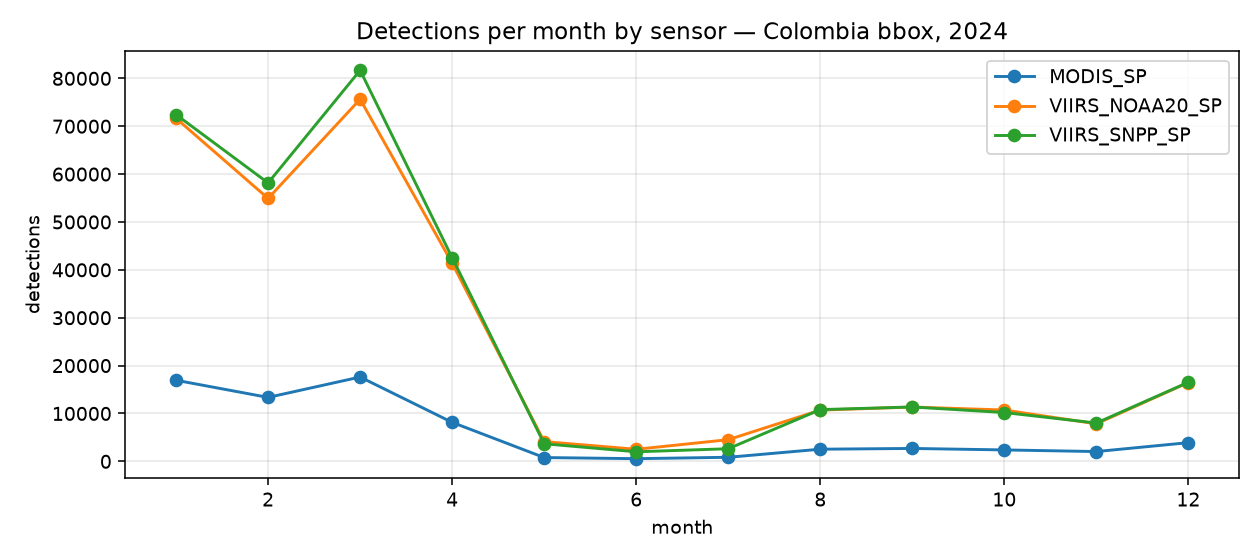
\includegraphics[width=0.92\textwidth]{../figures/sensor_seasonality_2024.png}
\caption{Detections per month and sensor, Colombia bounding box, 2024. January--April carries about
76\,\% of the year; May--June collapses by more than an order of magnitude.}
\end{figure}

\begin{figure}[h]
\centering
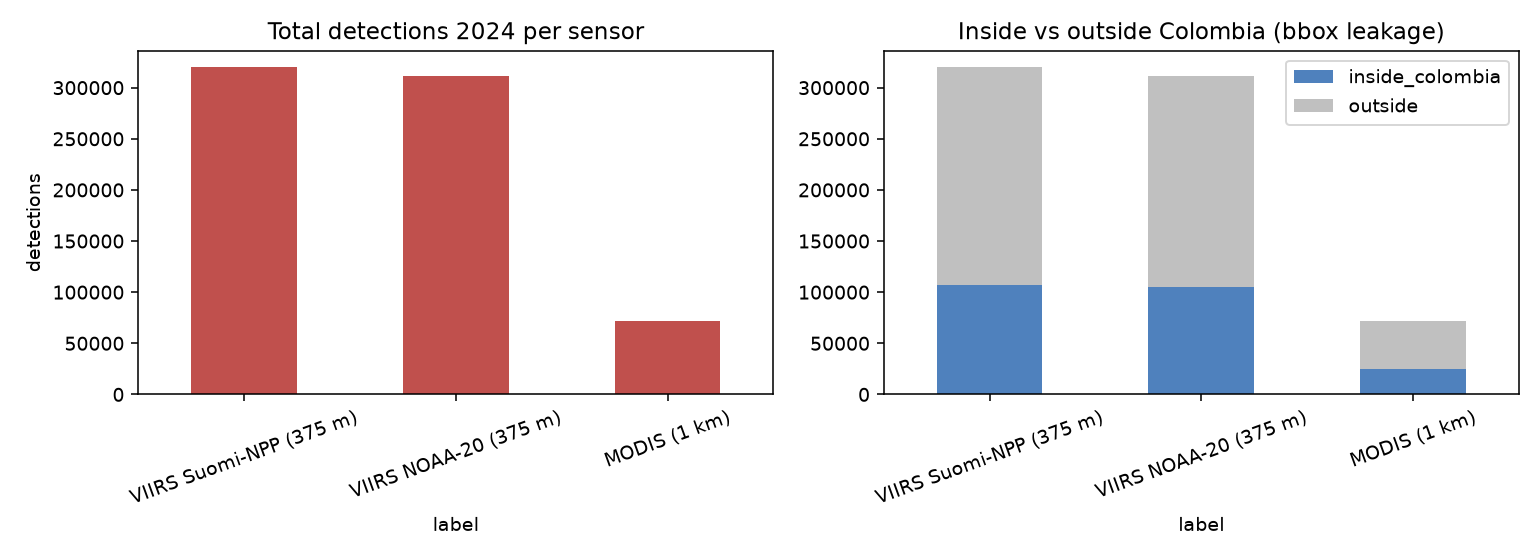
\includegraphics[width=0.98\textwidth]{../figures/sensor_volume_and_bbox_2024.png}
\caption{Total volume per sensor (left) and the share of records that are actually Colombian (right).}
\end{figure}

\paragraph{The second discontinuity: the weather model.} Open-Meteo documents that data from 2017
onwards uses newer 9~km models, while ERA5 is 0.25$^\circ$ and ERA5-Land 0.1$^\circ$. A baseline that
crosses 2017 therefore mixes model resolutions, exactly as a fire baseline mixes sensors. Both
discontinuities are treated the same way: baseline per era, and the choice of ERA5 as the fixed
model is recorded as a project decision.

\section{Overlap verification}

Five candidate pairs were extracted programmatically: NOAA-20 and NOAA-21 detections on the same
day, within 2~km of each other. They describe the same real fire.

\begin{table}[h]
\centering
\small
\begin{tabular}{lrrrrrrr}
\toprule
\textbf{Date} & \textbf{N20 time} & \textbf{N21 time} & \textbf{N20 FRP} & \textbf{N21 FRP} & \textbf{Distance} & \textbf{N20 conf} & \textbf{N21 conf} \\
\midrule
2026-11-10 & 07:01 & 06:03 & 2.48 & 2.70 & 0.07 km & n & n \\
2026-11-10 & 06:44 & 06:03 & 3.76 & 2.46 & 0.16 km & n & n \\
2026-11-10 & 06:24 & 06:03 & 1.21 & 2.43 & 0.30 km & n & n \\
2026-11-10 & 06:05 & 06:03 & 1.97 & 1.92 & 0.26 km & n & n \\
2026-11-10 & 06:41 & 06:03 & 1.50 & 1.50 & 0.12 km & n & n \\
\bottomrule
\end{tabular}
\caption{The same fire, two records: what differs is time, position, FRP and sometimes confidence.}
\end{table}

In every pair the timestamp differs (different overpass), the position differs by up to $\sim$300~m
(geolocation spread), the FRP differs (different pixel footprint), and the confidence code may
differ. What does not exist in any source is an identifier: it has to be constructed by the
ingestion layer. This is the empirical basis for the \code{fire\_event} table.

Because the assigned sources come from only two providers, cross-validation is done at the
\emph{processing} and \emph{model} level --- NRT against SP for the same date, ERA5 against the
forecast product for the same hour, ERA5 0.25$^\circ$ against the 9~km model --- rather than across
independent providers.

\section{Canonical mapping}

Every source field is mapped to the canonical event model
(\code{event\_id}, \code{source}, \code{event\_type}, \code{timestamp}, \code{latitude},
\code{longitude}, \code{severity}, \code{raw\_reference}).

\begin{table}[h]
\centering
\small
\begin{tabular}{L{3.6cm}L{4.4cm}L{6.8cm}}
\toprule
\textbf{Canonical field} & \textbf{Source field} & \textbf{Rule} \\
\midrule
\code{observed\_at} & \code{acq\_date} + \code{acq\_time} & Build an explicit UTC timestamp; \code{acq\_time} is HHMM without zero padding \\
\code{latitude}, \code{longitude} & \code{latitude}, \code{longitude} & WGS84, decimal degrees, as delivered \\
\code{severity} & \code{frp} & MW \\
\code{event\_id} & --- & Deterministic hash of source + rounded position + timestamp; never a serial \\
\code{raw\_reference} & --- & Path of the unmodified response + line number or record id \\
\bottomrule
\end{tabular}
\caption{Mapping for the fire sources (F1, F3).}
\end{table}

\paragraph{The weather sources do not fit the event model.} A weather value is a sample of a
continuous field at a location and time, not a discrete event. Only \code{observed\_at},
\code{latitude}, \code{longitude} (region centroid) and \code{raw\_reference} map onto
\code{event}; the measurements live in \code{weather\_observation}, in long format (one row per
variable), with the model and grid resolution recorded.

\subsection{Domain tables}

\begin{itemize}
  \item \code{region} --- 33 units: \code{region\_id}, name, level, centroid, geometry, source.
  \item \code{fire\_detection} --- hazard-specific attributes: \code{brightness},
        \code{bright\_ti4}, \code{bright\_ti5}, \code{frp}, \code{confidence\_raw},
        \code{confidence\_norm}, \code{satellite}, \code{instrument}, \code{scan}, \code{track},
        \code{daynight}, \code{product\_version}.
  \item \code{fire\_event} --- the grouping of detections: \code{first\_seen}, \code{last\_seen},
        centroid, \code{n\_detections}, \code{frp\_sum}, \code{frp\_max}, \code{sensor\_set},
        \code{cluster\_params}.
  \item \code{weather\_observation} --- \code{region\_id}, \code{observed\_at}, \code{variable},
        \code{value}, \code{unit}, \code{source}, \code{model}, \code{grid\_resolution\_deg}.
  \item \code{ingestion\_run} --- operational state: source, partition, mode, status, watermark
        before and after, row counts, error message.
\end{itemize}

\begin{figure}[H]
\centering
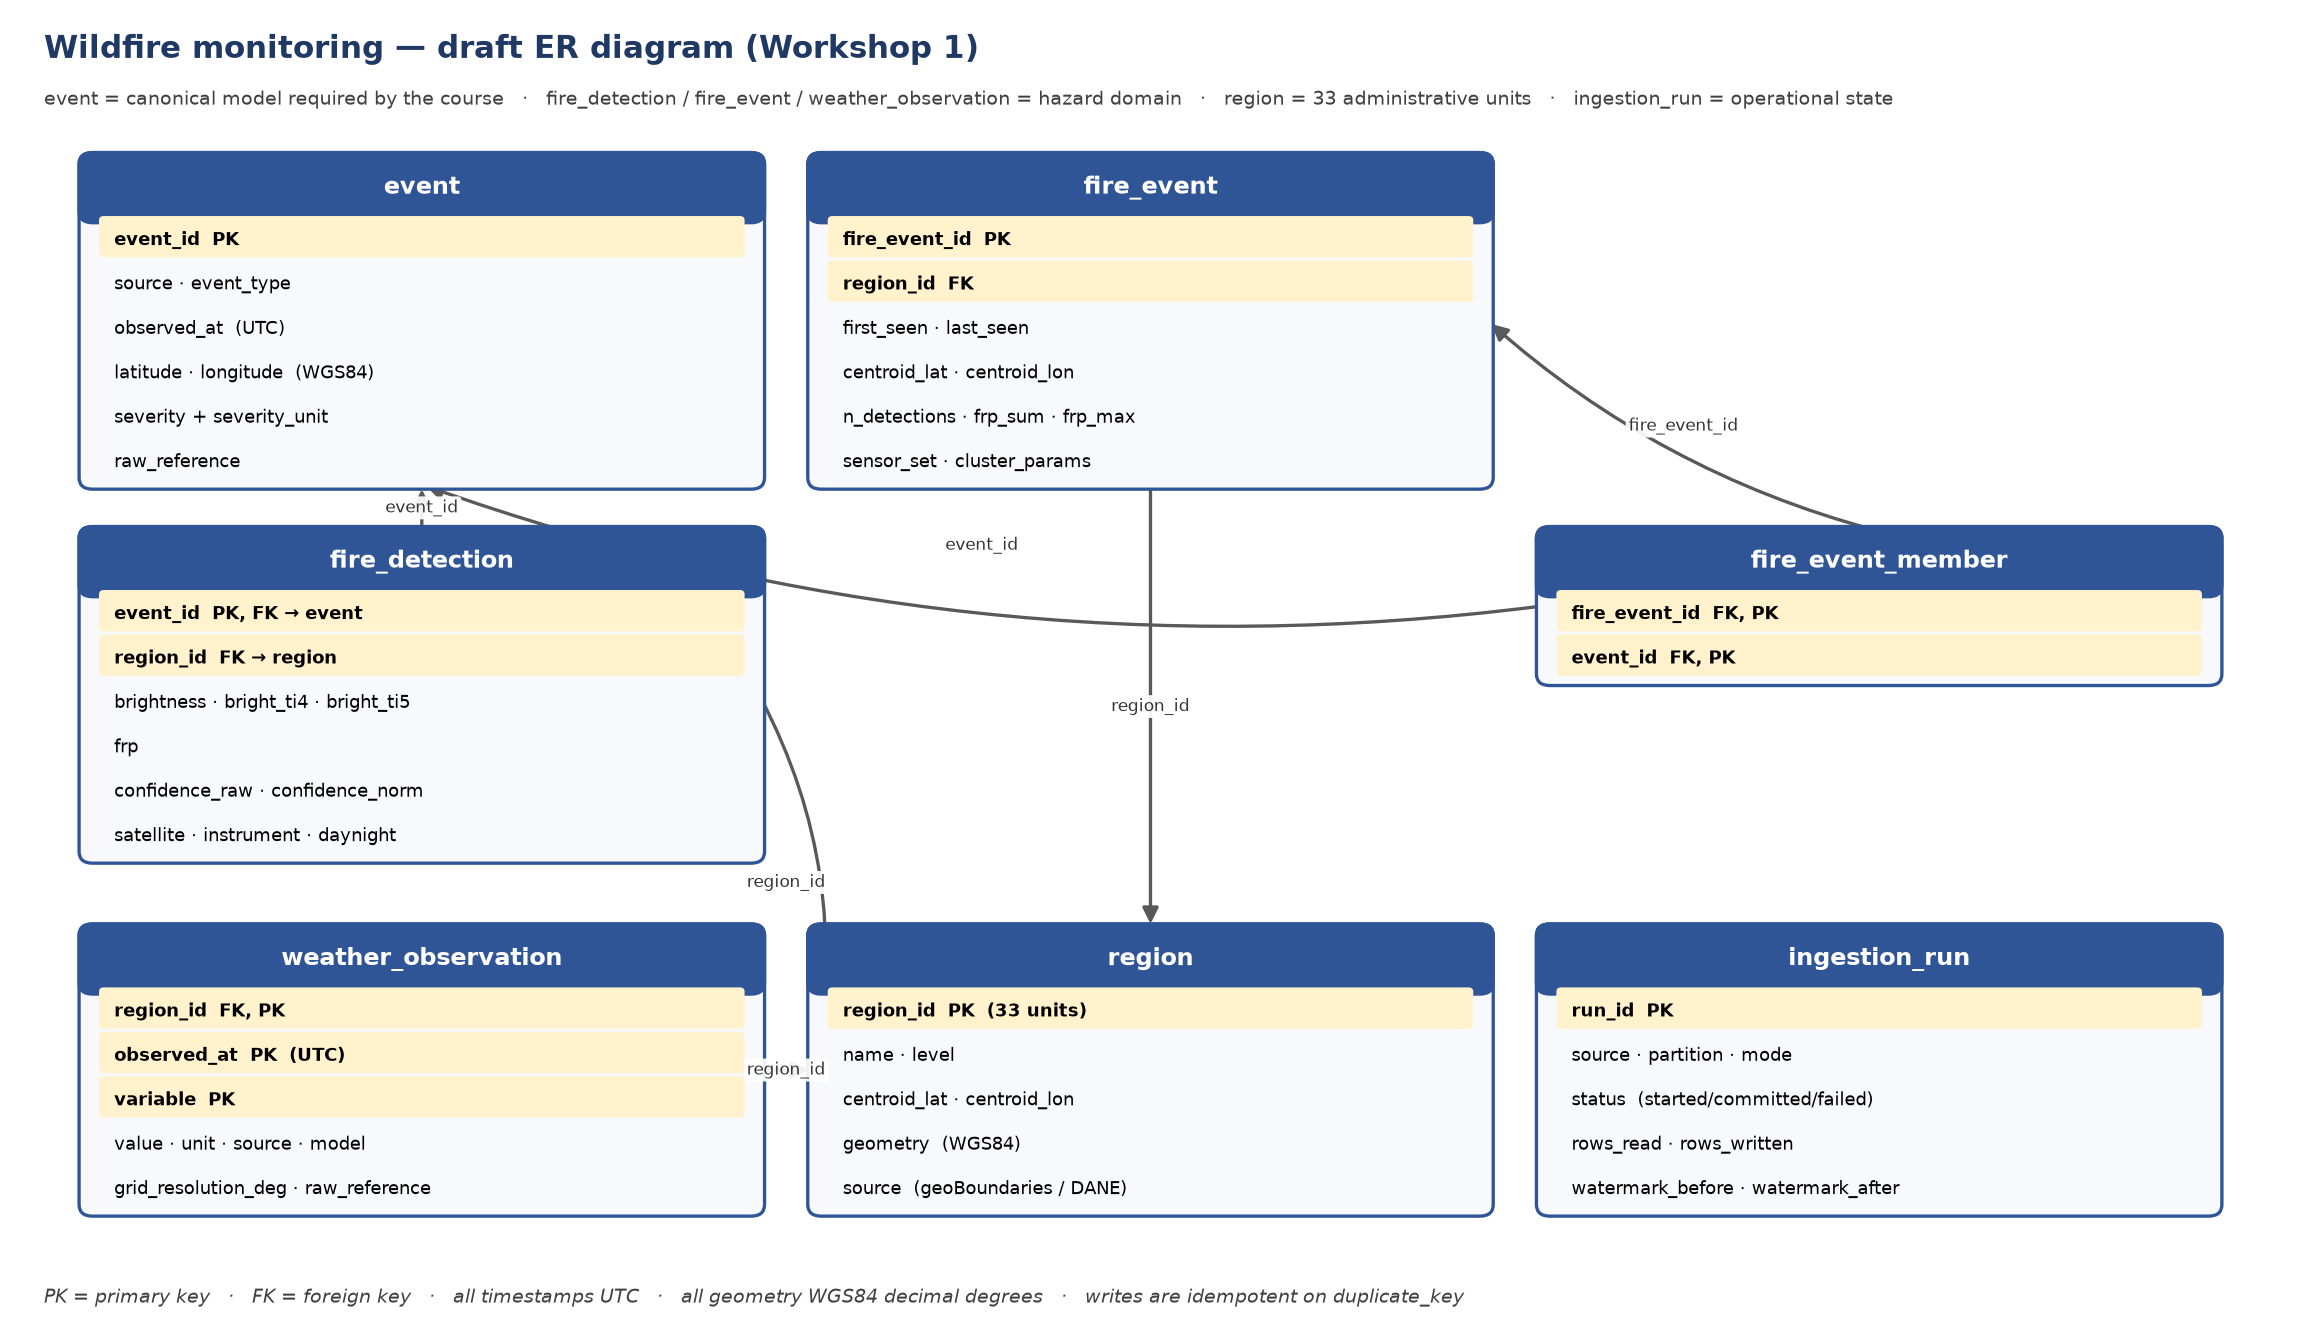
\includegraphics[width=\textwidth]{../figures/er_diagram.png}
\caption{Draft entity-relationship diagram. \code{event} is the canonical model required by the
course; \code{fire\_detection}, \code{fire\_event} and \code{weather\_observation} are the
hazard-specific tables; \code{region} is the reference layer that makes the ``per region''
indicator possible; \code{ingestion\_run} makes the pipeline restartable.}
\label{fig:er}
\end{figure}

The diagram in Figure~\ref{fig:er} also encodes the central modelling tension: weather is a
\emph{series} attached to a region and a time, not an event attached to a coordinate, which is
why it needs its own table rather than a wider \code{event}.

\subsection{Grouping detections into fire events}

This is the main challenge of the workshop. With 44.5\,\% of rows sharing a $\sim$1~km cell, a raw
count measures the number of pixels observed, not the number of fires. The proposed rule:

\begin{itemize}
  \item \textbf{Space:} $\varepsilon_{space} \approx 1.5$--$2$~km, because the VIIRS footprint is
        375~m but cross-sensor geolocation spread reaches $\sim$1~km.
  \item \textbf{Time:} $\varepsilon_{time} \approx 24$~h with connected-component chaining, because
        a fire burns for days and must remain \emph{one} event.
  \item \textbf{Identifier:} hash of the rounded centroid plus \code{first\_seen}, so the grouping is
        reproducible and idempotent.
  \item \textbf{Metrics:} report three --- detection count, grouped event count and $\Sigma$FRP ---
        and state which one the indicator uses.
\end{itemize}

\subsection{Normalisation rules}

All timestamps are UTC (\code{TIMESTAMPTZ}); coordinates are WGS84 decimal degrees validated against
the region polygons; FRP is in MW; precipitation in mm; wind in km/h; temperature in $^\circ$C; VPD in
kPa. Confidence is harmonised to 0--100 with a documented mapping table. Units are declared per
column and never inferred at read time.

\section{Ingestion contract}

\begin{table}[h]
\centering
\small
\begin{tabular}{L{2.3cm}L{4.2cm}L{4.4cm}L{4.0cm}}
\toprule
\textbf{Source} & \textbf{Historical strategy} & \textbf{Incremental strategy} & \textbf{Duplicate key} \\
\midrule
F1 archive & Partition by year and sensor; 5-day windows through the API; one file per window; permanent cache with checksum & none (archive is bounded) & source, lat, lon, \code{acq\_date}, \code{acq\_time}, satellite \\
F2 ERA5 & Partition by year; one request per month with all 33 centroids; \code{timezone=UTC} & none & \code{region\_id}, \code{observed\_at}, variable, model \\
F3 FIRMS NRT & none & Watermark = max(\code{acq\_date}, \code{acq\_time}) in UTC; poll every 3~h (NRT latency); \code{DAY\_RANGE=2} with a 1-day overlap; seven days requires two calls & source, lat, lon, \code{acq\_date}, \code{acq\_time}, satellite \\
F4 forecast & none & Hourly; \code{past\_days=7} and \code{forecast\_days=7} in one call; 48~h overlap; \code{timezone=UTC} & \code{region\_id}, \code{observed\_at}, variable \\
\bottomrule
\end{tabular}
\caption{Per-source contracts.}
\end{table}

\paragraph{Correctness when a run fails halfway.} Writes are idempotent on the duplicate key
(\code{INSERT \ldots ON CONFLICT DO NOTHING}); each partition is loaded in its own transaction; the
watermark advances \emph{only} after the partition is committed; and \code{ingestion\_run} records
\code{started}, \code{committed} or \code{failed} with the watermark before and after. The overlap window
is the recovery policy, not redundancy: if the 12:00 poll fails, the 15:00 poll with
\code{DAY\_RANGE=2} recovers the lost window. The partitioned historical pull is resumable for the
same reason --- windows already on disk are reported as \code{cached} in the manifest and skipped.

\paragraph{A source that revises its own past.} Near-real-time records are replaced by
standard-processing records with roughly a five-month lag. Any design that assumes historical
immutability is wrong: the contract includes a correction window of five months during which the
same date is re-queried.

\section{Project definition}

\subsection{Functional user}
\textbf{Role:} risk analyst at a departmental emergency-management office.
\textbf{Profile:} works with weekly incident summaries, has no GIS tooling, needs a defensible
number to justify resource allocation before a dry-season peak.
\textbf{Decisions supported:} which departments to inspect first, whether the current week is worse
than a normal week given the rainfall, and how stale the underlying data is.
\textbf{Why a dashboard:} the analyst cannot join satellite detections with reanalysis weather by
hand, and doing so monthly does not scale past a handful of departments.

\subsection{User stories (MoSCoW)}

\begin{table}[h]
\centering
\small
\begin{tabular}{L{1.3cm}L{13.7cm}}
\toprule
\textbf{Priority} & \textbf{Story} \\
\midrule
Must & As an emergency-management analyst, I want the detections of the last 24 hours per department, so that I can prioritise field verification. \\
Must & As an analyst, I want the last 7 days compared with the historical average for the same calendar window, so that I know whether the activity is unusual. \\
Must & As a risk researcher, I want the data freshness and the covered window displayed, so that I know whether I can trust the board. \\
Should & As an analyst, I want to filter by confidence level and by day/night, so that I can discard false positives. \\
Should & As a local authority, I want a ranking of departments by anomaly, so that I can allocate resources. \\
Could & As a journalist, I want to export the raw reference of a detection, so that I can cite the source. \\
Could & As a researcher, I want the monthly sequence of detections per sensor, so that I can separate instrument effects from real trends. \\
\bottomrule
\end{tabular}
\caption{Seven user stories, prioritised. Monitoring, analysis and trust are all covered.}
\end{table}

\subsection{Indicator proposal}

The indicator is \textbf{conditioned on weather}, because the assignment asks for activity
``unusual relative to historical patterns and weather conditions''.

\begin{enumerate}
  \item \textbf{Panel:} one row per region-day with detections, grouped fire events, $\Sigma$FRP and
        weather (temperature, minimum relative humidity, accumulated precipitation over 7 and 30
        days, wind, VPD, soil moisture).
  \item \textbf{Expected value:} estimate $\mathrm{E}[\mathrm{detections} \mid \mathrm{weather}]$ with a
        Poisson or negative-binomial regression, or --- if time is short --- by stratifying into
        bins of dry/wet $\times$ hot/cool $\times$ windy/calm.
  \item \textbf{Anomaly:} observed / expected, plus the percentile of the residual within the same
        region and calendar window.
  \item \textbf{Output scale:} five levels --- Very low (below P10), Low (P10--P25), Normal
        (P25--P75), Elevated (P75--P90), Extreme (above P90).
  \item \textbf{Validation:} the index must spike in January 2024 (Bogotá and Cundinamarca), in the
        2019 Amazon season, and must \emph{not} spike in a wet control year.
\end{enumerate}

The assumption behind the conditioning was already tested on real data: for 2024, daily detections
correlate \textbf{+0.83} with VPD, \textbf{$-$0.69} with seven-day accumulated precipitation and
\textbf{+0.72} with maximum temperature. Two regions with different rainfall cannot be compared by
raw counts; the difference would be weather, not anomaly.

\begin{figure}[h]
\centering
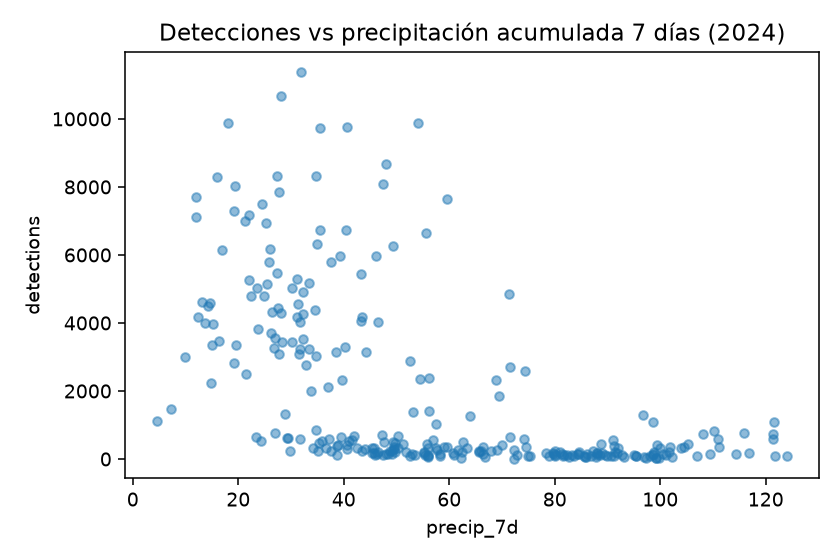
\includegraphics[width=0.66\textwidth]{../figures/detections_vs_precip.png}
\caption{Detections against seven-day accumulated precipitation, 2024. The negative relation is the
empirical justification for a weather-conditioned baseline.}
\end{figure}

\paragraph{What the indicator is not.} It describes anomalous observed activity. It is not a forecast,
not a fire-danger index, and not the Canadian FWI --- implementing FWI is out of scope for this
workshop and, if done later, must be described as an inspired composite rather than a standard one.

\subsection{Risks and mitigation}

\begin{table}[h]
\centering
\small
\begin{tabular}{L{5.4cm}L{9.4cm}}
\toprule
\textbf{Risk} & \textbf{Mitigation} \\
\midrule
Counting the sensor change as an anomaly (the dominant risk of this workshop) & Per-sensor baseline; harmonise only across the VIIRS pair (factor 1.026); document the effect with the 2024 figures \\
Sensor end of life (S-NPP ceased 2026-11-02) & NOAA-20/21 for the incremental stream; frozen sensors only as archive \\
Rate limits (5000 transactions / 10 min; 10\,000 calls/day) & Partitioning, permanent cache, exponential backoff, resumable manifest \\
Open-Meteo free tier exhausted (600 calls/min) & One call with 33 coordinates instead of 33 calls; batch by month \\
Schema change between MODIS and VIIRS (columns differ) & Early normalisation into \code{fire\_detection}; fixtures covering both sensors \\
Bounding box includes five countries & Mandatory point-in-polygon filter before aggregation (33.7\,\% are Colombian) \\
Days without overpass (clouds, satellite failure) & \code{data\_availability} / \code{missing\_data} endpoints; ``no coverage'' is never stored as ``zero fires'' \\
Ambiguous identifiers (no native event id) & Deterministic composite identifier and a grouped \code{fire\_event} table \\
License and attribution & NASA EOSDIS citation, Open-Meteo CC-BY 4.0, plus a licence row per source in the documentation \\
\bottomrule
\end{tabular}
\caption{Risks and mitigations.}
\end{table}

\subsection{Architecture overview}
Four layers follow the reference architecture of the course project, adapted to this hazard:
\textbf{(1) acquisition} --- one module per source under \code{src/sources/}, driven by
\code{config/sources.yaml}, with caching and watermark state; \textbf{(2) normalisation} --- unit,
timezone, confidence and region assignment under \code{src/normalization/};
\textbf{(3) storage} --- \code{event}, \code{fire\_detection}, \code{fire\_event}, \code{region},
\code{weather\_observation} and \code{ingestion\_run} in \code{sql/schema.sql};
\textbf{(4) presentation} --- a Dash application in \code{dashboard/} fed by the region-day panel.
\code{ingest.py} is the command-line entry point that orchestrates the layers; at this stage it is a
stub that resolves configuration and reports the declared sources.

\section{Conclusions and limitations}

\begin{itemize}
  \item The four sources were validated with real queries; the archive alone accounts for
        703\,633 detections in 2024, so the volume justifies the partitioned design.
  \item The instrument discontinuity is quantified, not merely acknowledged: 8.8$\times$ in count and
        3.57$\times$ in mean FRP between MODIS and VIIRS, against 2.6\,\% between the two VIIRS
        sensors.
  \item Only a third of the records returned by the bounding box are Colombian, and the share moves
        with the season.
  \item Weather is a first-class source and a modelling constraint: it is a series, it must be
        forced to UTC, its model changes in 2017, and it explains most of the seasonal variance.
  \item \textbf{Limitations:} the weather baseline is a centroid approximation, not an area average;
        ERA5 latency means the most recent days come from a different product, whose seam is
        declared rather than hidden; NOAA-21 history is too short to anchor the baseline; and the
        grouping thresholds are proposed values that still have to be tuned and validated against
        known fires.
\end{itemize}

\section*{References and attribution}
\small
\begin{itemize}
  \item NASA FIRMS / LANCE, NASA EOSDIS. Archive and area API documentation:
        \url{https://firms.modaps.eosdis.nasa.gov/api/area/} and
        \url{https://firms.modaps.eosdis.nasa.gov/download/}
  \item Open-Meteo, Historical Weather API (ERA5, ECMWF Copernicus) and Forecast API:
        \url{https://open-meteo.com/en/docs/historical-weather-api}; terms:
        \url{https://open-meteo.com/en/terms}
  \item geoBoundaries, \code{gbOpen/COL/ADM1} (ODbL 1.0), \url{https://www.geoboundaries.org}
  \item DANE, Marco Geoestadístico Nacional (official alternative for the region layer).
\end{itemize}

\end{document}
